\chapter{Garment Analysis}
\label{garment_analysis}

This chapter explains in detail the gament analysis that our algorithm performs to the garment data previously segmented. The contour of the garment is extracted, and a Watershed segmentation algorithm is applied to find the different overlapped patches.

\section{Contour extraction}
From the mask obtained in the previous step (section \ref{garment_segmentation_mask}) a blob labeling algorithm is applied to detect the garment outline. This outline will be used in later steps to obtain the candidates to be a fold.

The contour extraction method used is a Topological Analysis by Border Following algorithm developed by Suzuki and Abe\comment{[ref to suzuki85]}. This is a widely used algorithm for connected-component labeling and countour finding. Only external contours were retrieved. A simple chain approximation was then applied to reduce the number of points that describe the contours, storing only the endpoints of the different segments.

Due to noise, sometimes some small blobs appear in segmentation masks, so the extracted contour with the highest area was selected as garment. This way, those small blobs were discarded.

After obtaining the garment contour, it is processed, as we want to obtain a further simplified garment outline. We assume the fold line has a very high probability of lying in the garment outline. Therefore, this contour will represent all the candidate segments that \comment{could be folds.} The Ramer–Douglas–Peucker algorithm \comment{[ref to article]} is applied to obtain the simplified outline. This algorithm recursively divides the contour in segments by choosing the \comment{...}

\section{Watershed segmentation}

Watershed is a segmentation algorithm that considers a greyscale image as a topological surface where high intensity pixels correspond to peaks and hills, and low intensity pixels are equivalent to valleys. The algorithm fills the surface pouring water at each isolated valley. As the water level rises, the water from different sources will start to merge. To prevent them from merging, the algorithm constructs barriers at the merging regions, and continues this process of adding water and building barriers until all the peaks have been flooded. The resulting barriers are the segmentation result, where each region enclosed correspond to a segmented item.

\comment{(Here it would be great to add a figure of the example, such as opencv's coins)}

As in practise flooding using local minima as makers leads to over- segmentation, an enhanced version of this algorithm allows the user to specify other criteria for selecting the seed points. In this work, the gradient of the greyscale depth-image was calculated and regions where the gradient has a low value were selected. These regions correspond to homogeneous and continous regions, which are good candidates to be used as markers.

\begin{figure}[thpb]
    \centering
    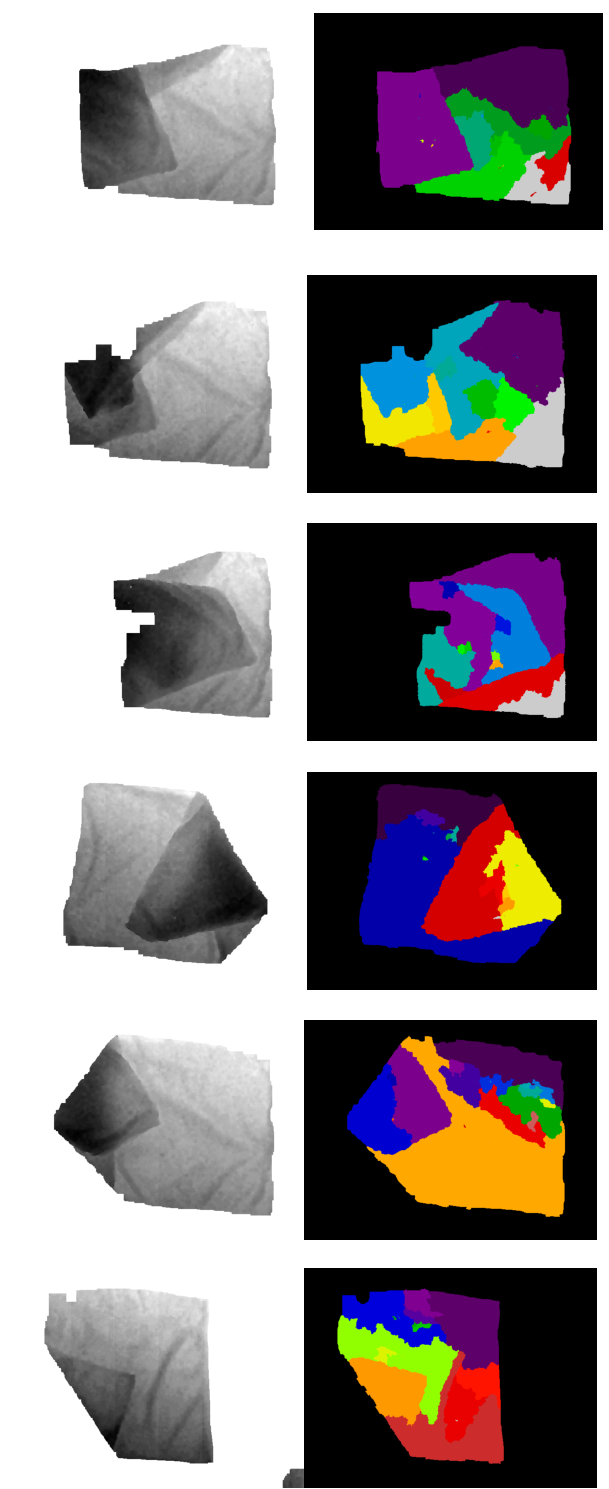
\includegraphics[width=0.38\textwidth]{figures/colour_garment.pdf}
    \caption{On the left side, the grayscale images are shown. The grey level is related to the height of the point as detected by the RGB-D sensor. On the right side, the labeled image returned by watershed algorithm is presented, where each color represents a region of similar height.}
    \label{colour_garment}
\end{figure}